\documentclass[aspectratio=43,9pt]{beamer}
%
\usepackage{graphicx,tikz}
%
\usetheme{Boadilla}
%
\graphicspath{{./figures}}
%
\let\Tiny=\tiny%			% to avoid warnings about font size
%\usepackage{lmodern}%		% alternative method to avoid these warnings
%
\catcode`~=11 % make LaTeX treat tilde (~) like a normal character
\newcommand{\urltilde}{\hbox{~}}
\catcode`~=13 % revert back to treating tilde (~) as an active character
%
% misc commands
\newcommand{\bm}[1]{\mathbf{#1}}
\newcommand{\bs}[1]{\boldsymbol{#1}}
\newenvironment{myitemize}[1]{\vspace{#1}\begin{itemize}\setlength\itemsep{#1}}{\end{itemize}}
%
% pgf markers
\usepgflibrary{plotmarks}
%
\setbeamertemplate{footline}
{
  \leavevmode%
  \hbox{%
  \begin{beamercolorbox}[wd=.8\paperwidth,ht=2.25ex,dp=1ex,left]{author in head/foot}%
    \usebeamerfont{author in head/foot}\hspace*{4em}\inserttitle
  \end{beamercolorbox}%
  \begin{beamercolorbox}[wd=.2\paperwidth,ht=2.25ex,dp=1ex,right]{author in head/foot}%
    \usebeamerfont{author in head/foot}\insertframenumber{} / \inserttotalframenumber\hspace*{1ex}
  \end{beamercolorbox}}%
  \vskip0pt%
}
%
\setbeamertemplate{navigation symbols}{}
%
\setbeamertemplate{frametitle}
{%
	\begin{minipage}{.9\paperwidth}
		\vspace*{1ex}%
		\flushright%
		%\bfseries
		\LARGE%
		\insertframetitle%
	\end{minipage}%
}
%
\setbeamertemplate{title page}{
	\begin{center}
		\vspace*{2ex}
		\usebeamercolor[fg]{frametitle}{%
			\Large%
			Numerical Techniques 2024--2025\\[2ex]
			%
			\LARGE%
			\inserttitle
		}\\[6ex]
		\usebeamercolor[fg]{normal text}{%
			Daan Degrauwe\\[1ex]
			\texttt{daan.degrauwe@meteo.be}\\[4ex]
			Postgraduate Studies in Weather and Climate Modeling\\[1ex]
			Ghent University
		}
	\end{center}
}
%
\newcommand{\ft}[2]{{\textstyle\frac{#1}{#2}}}
%
% increase space around equations
\makeatletter
\g@addto@macro\normalsize{%
	\setlength{\abovedisplayskip}{3ex}%
	\setlength{\belowdisplayskip}{3ex}%
	\setlength{\abovedisplayshortskip}{3ex}%
	\setlength{\belowdisplayshortskip}{3ex}%
}%
\makeatother
%

%
\title{Student projects}%
%
%%%%%%%%%%%%%%%%%%%%%%%%%%%%%%%%%%%%%%%%%%%%%%%%%%%%%%%%%%%%%%%%%%%%%%
%
\begin{document}
%
%%%%%%%%%%%%%%%%%%%%%%%%%%%%%%%%%%%%%%%%%%%%%%%%%%%%%%%%%%%%%%%%%%%%%%%%%%%%%%%%%%%%%%%%%%%%%%%%%%%%
%
\begin{frame}[plain]
	\titlepage
\end{frame}
%
%\begin{frame}
%
%[CHEBYSHEV: EXPLAIN THAT NOT THAT DIFFERENT FROM FOURIER: T\_n(cos(theta)) = cos(n.theta) ]
%[CHEBYSHEV: REF. TO NUMERICAL RECIPES]
%[Explain Davies perfect model experiments better, perhaps in separate document]
%[Provide Pierre's work on background state as reference for SI-SWE]
%
%\end{frame}
%
%%%%%%%%%%%%%%%%%%%%%%%%%%%%%%%%%%%%%%%%%%%%%%%%%%%%%%%%%%%%%%%%%%%%%%
%
\begin{frame}
	%
	\frametitle{General idea}
	%
	\begin{center}
		\bf Starting from a simple model, apply some\\
		of the techniques from this course.
	\end{center}
	%
	\par\vspace*{4ex}
	General remarks:
	%
	\begin{myitemize}{1ex}
		\item no course on Python; no course on complex algebra;\\ask for help!
		\item open assignment: no exact solution $+$ discussion is more important than results
		\item the purpose is you \emph{learn} something
		\item try to trigger strange/unwanted phenomena, and discuss solutions.
		\item you can propose a topic yourself.
	\end{myitemize}
	%
\end{frame}
%
%%%%%%%%%%%%%%%%%%%%%%%%%%%%%%%%%%%%%%%%%%%%%%%%%%%%%%%%%%%%%%%%%%%%%%
%
\begin{frame}
	%
	\frametitle{Shallow Water Equations}
	%
	\begin{center}
		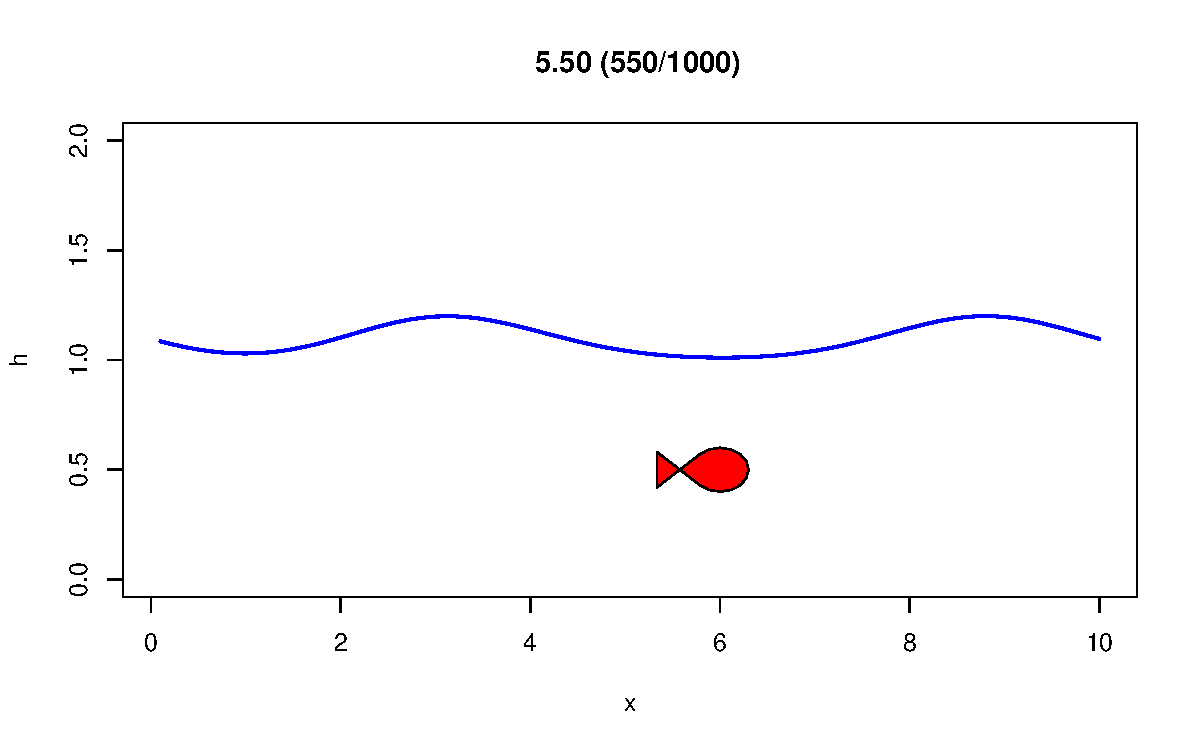
\includegraphics[width=9cm]{swe1D}
	\end{center}
	%
\end{frame}
%
%%%%%%%%%%%%%%%%%%%%%%%%%%%%%%%%%%%%%%%%%%%%%%%%%%%%%%%%%%%%%%%%%%%%%%
%
\begin{frame}
	%
	\frametitle{Shallow Water Equations}
	%
	The linearized 1D shallow water equations (SWE) are given by:
	%
	\begin{align*}
		\frac{\partial u}{\partial t}+U\frac{\partial u}{\partial x}+g\frac{\partial h}{\partial x}&=0\\
		\frac{\partial h}{\partial t}+H\frac{\partial u}{\partial x}+U\frac{\partial h}{\partial x}&=0
	\end{align*}
	%
	where $g$ is gravity, $U$ and $H$ are the constant basic-state velocity and water height, and $u(x,t)$ and $h(x,t)$ are the perturbations on the velocity and the water height.
	%
\end{frame}
%
%%%%%%%%%%%%%%%%%%%%%%%%%%%%%%%%%%%%%%%%%%%%%%%%%%%%%%%%%%%%%%%%%%%%%%
%
\begin{frame}
	%
	\frametitle{Shallow Water Equations}
	%
	The current model is very simple:
	%
	\begin{myitemize}{1ex}
		\item Leapfrog time integration
		\item Second-order centered space differencing
		\item Periodic boundary conditions
	\end{myitemize}
	%
	{\vspace*{4ex}\bfseries Student projects}:
	%
	\begin{myitemize}{1ex}
		\item[1.] Stagger $u$ and $h$
		\item[2.] Compare with nonlinear model
		\item[3.] Transform into spectral model with Fourier decomposition
		\item[4.] Transform into spectral model with Chebyshev decomposition\\[1mm]
			\quad J.P. Boyd, \emph{Chebyshev and Fourier Spectral Methods}\\
		\item[5.] Study Laplace transform integration\\[1mm]
			\quad\parbox{.9\textwidth}{Clancy and Lynch, 2011, QJRMS 137,\\\emph{Laplace transform integration of the shallow-water equations}}\\[1mm]
		%\item[6.] Study effect of lateral boundary conditions with Davies relaxation
	\end{myitemize}
	%
\end{frame}
%
%%%%%%%%%%%%%%%%%%%%%%%%%%%%%%%%%%%%%%%%%%%%%%%%%%%%%%%%%%%%%%%%%%%%%%
%
\begin{frame}
	%
	\frametitle{Barotropic Vorticity Equation}
	%
	\begin{center}
		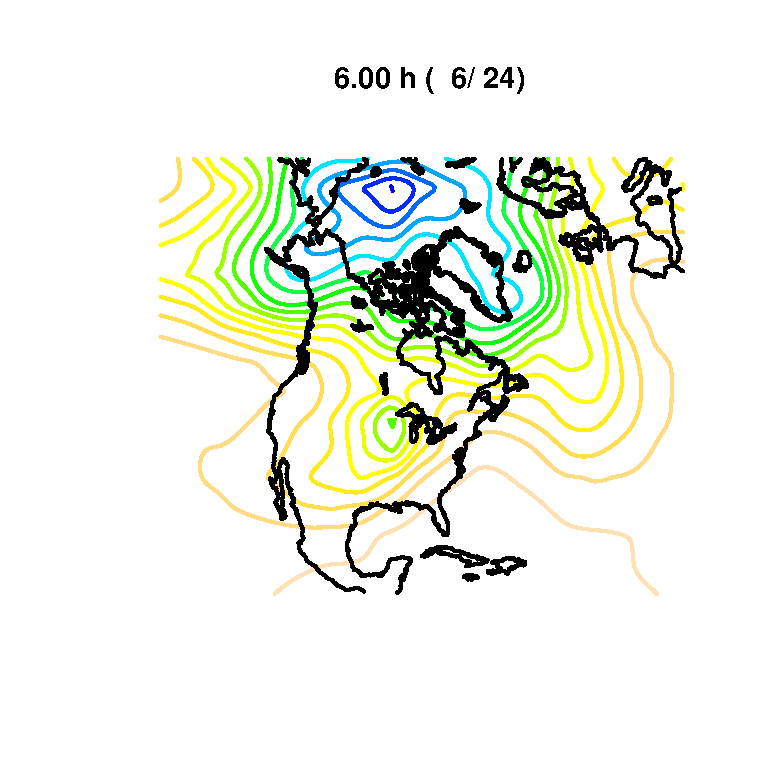
\includegraphics[width=7cm]{barovort}
	\end{center}
	%
\end{frame}
%
%%%%%%%%%%%%%%%%%%%%%%%%%%%%%%%%%%%%%%%%%%%%%%%%%%%%%%%%%%%%%%%%%%%%%%
%
\begin{frame}
	%
	\frametitle{Barotropic Vorticity Equation}
	%
	\begin{myitemize}{2ex}
		\item The barotropic vorticity equation BVE is given by:
			%
			\begin{equation*}
				\frac{\partial \zeta}{\partial t}+\bm u\cdot\nabla\zeta=0
			\end{equation*}
			%
			where $\zeta$ is the vorticity, and $\bm u$ is the geostrophic wind, given by
			%
			\begin{align*}
				\bm u&=\bm k\times\nabla\psi		&		\nabla^2\psi&=\zeta
			\end{align*}
			%
		\item Writing everything in terms of the streamfunction $\psi$, the BVE becomes
			%
			\begin{equation*}
				\frac{\partial\nabla^2\psi}{\partial t}+J(\psi,\nabla^2\psi)=0
			\end{equation*}
			%
			where $J$ is the Jacobian operator:
			%
			\begin{equation*}
				J(p,q)=\frac{\partial p}{\partial x}\frac{\partial q}{\partial y}-\frac{\partial p}{\partial y}\frac{\partial q}{\partial x}
			\end{equation*}
			%
	\end{myitemize}
	%
\end{frame}
%
%%%%%%%%%%%%%%%%%%%%%%%%%%%%%%%%%%%%%%%%%%%%%%%%%%%%%%%%%%%%%%%%%%%%%%
%
\begin{frame}
	%
	\frametitle{Some background info}
	%
	\begin{myitemize}{2ex}
		\item This model was used for the first numerical weather prediction in 1950 on the ENIAC computer
			%
			\begin{center}
				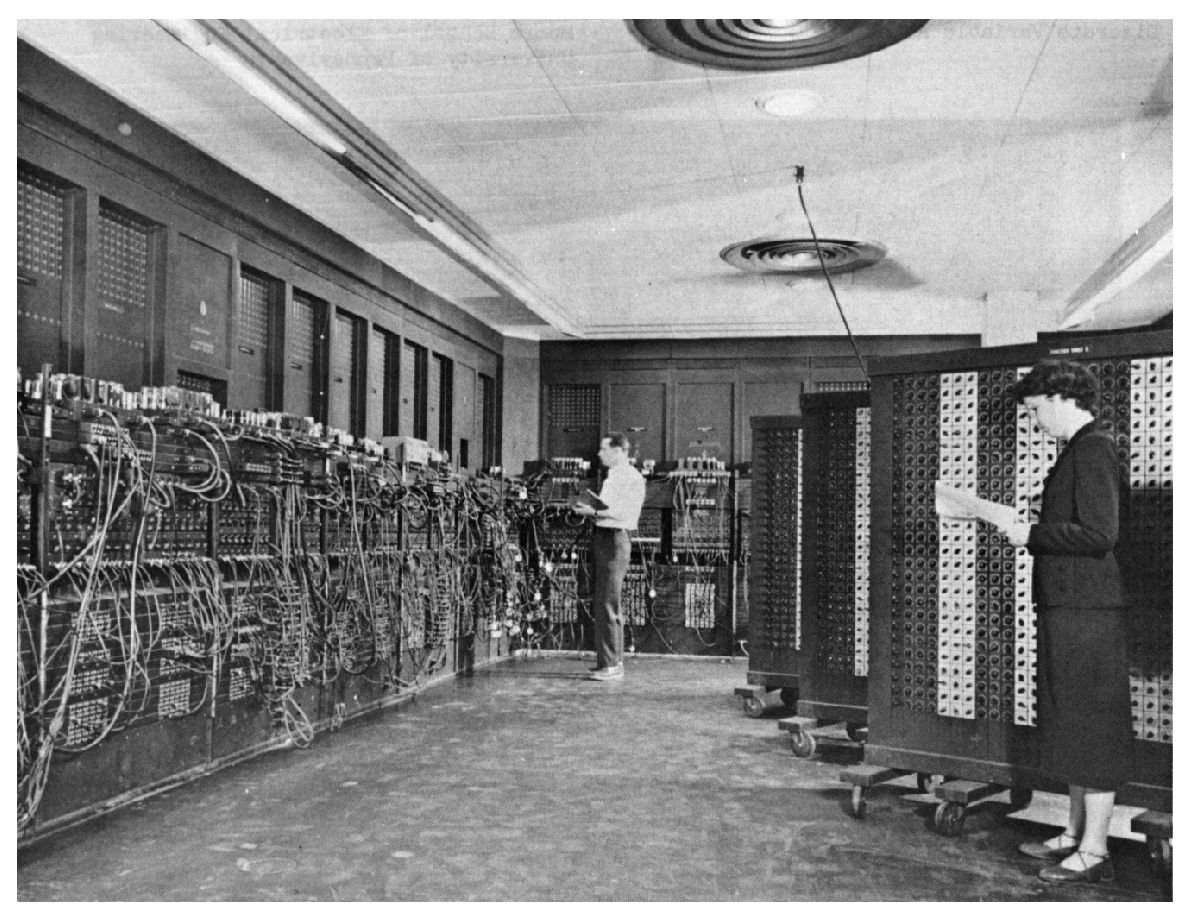
\includegraphics[width=5cm]{ENIAC}
			\end{center}
			%
		\item A 24-hour forecast took about 24h computing time
			%
	\end{myitemize}
	%
\end{frame}
%
%%%%%%%%%%%%%%%%%%%%%%%%%%%%%%%%%%%%%%%%%%%%%%%%%%%%%%%%%%%%%%%%%%%%%%
%
\begin{frame}
	%
	\frametitle{Original model}
	%
	The original (1950) model is characterized by:
	%
	\begin{myitemize}{1ex}
		\item a leapfrog time integration
			%
		\item second-order centered space differences
			%
		\item an expensive (pseudo-spectral) way to invert the Laplacian operator
			%
		\item heuristic boundary conditions:
			%
			\begin{myitemize}{1ex}
				\item $\frac{\partial \psi}{\partial t}=0$ on boundary
				\item $\frac{\partial \nabla^2 \psi}{\partial t}=0$ for entering fluid
			\end{myitemize}
			%
	\end{myitemize}
	Due to these boundary conditions and aliasing, the model is not stable.
	%
	\par\vspace*{4ex}
	The student's model is somewhat simplified:
	%
	\begin{myitemize}{1ex}
		\item Spectral inversion of Laplacian
		\item Periodic boundary conditions
		\item Coriolis effect removed
		\item Projection impact removed
	\end{myitemize}
	%
\end{frame}
%
%%%%%%%%%%%%%%%%%%%%%%%%%%%%%%%%%%%%%%%%%%%%%%%%%%%%%%%%%%%%%%%%%%%%%%
%
\begin{frame}
	%
	\frametitle{Improvements (student projects)}
	%
	General remark: lots of interesting aspects in this model, but you'll have to dig deeper to find them.
	%
	\par\vspace*{4ex}
	{\bf Student projects:}
	\begin{myitemize}{1ex}
		\item[6.] Semi-Lagrangian scheme
		\item[7.] High-resolution LAM nested in low-resolution LAM (coupling with Davies relaxation)
		\item[8.] Spectral model and avoiding aliasing
		\item[9.] Check energy cascade between large and small scales, and implement Arakawa Jacobian
	\end{myitemize}
	%
\end{frame}
%
%%%%%%%%%%%%%%%%%%%%%%%%%%%%%%%%%%%%%%%%%%%%%%%%%%%%%%%%%%%%%%%%%%%%%%
%
\begin{frame}
	%
	\frametitle{Practical aspects}
	%
	\begin{myitemize}{2ex}
		\item Groups of 2/3 persons
			%
		\item Pick a single topic (e.g. SWE-spectral); post your group + choice on Ufora forum.
			%
		\item Jupyter notebooks for SWE and BVE on Ufora.
			%
		\item More detailed background info (papers) on Ufora.
			%
		\item Support sessions: \textbf{4 and 11 December}, 16h00-17h30; come prepared!
			%
		\item Report (say 5--10 pp.): deadline Thursday 14 December.
		\item Presentation for other students: Monday 18 December.
	\end{myitemize}
	%
\end{frame}
%
%%%%%%%%%%%%%%%%%%%%%%%%%%%%%%%%%%%%%%%%%%%%%%%%%%%%%%%%%%%%%%%%%%%%%%
%
\end{document}
